\chapter{بررسی و ارزیابی}
در این فصل به ارزیابی‌ها و بررسی‌های انجام شده بر روی پروژه پرداخته خواهد شد.

\section{تست‌های واحد}
تست واحد\LTRfootnote{Unit Test} یکی از مهم‌ترین بخش‌های ارزیابی یک برنامه است. این مدل از ارزیابی به بررسی عملکرد یک واحد از برنامه می‌پردازد. یک واحد به معنی کوچک‌ترین بخش منزوی از یک برنامه ‌است که به صورت مستقل عمل می‌کند و ورودی و خروجی مشخصی دارد. این واحد می‌تواند بخشی از یک تابع، کل تابع و یا مجموعه‌ای از توابع باشد. از مزایای تست واحد، می‌توان به صحت سنجی عملکرد واحد‌ها نسبت به ورودی‌های مختلف اشاره کرد که کمک بسیار شایانی به اجرا‌های موفق می‌کند و ریسک عملکردهای دور از انتظار را بسیار کاهش می‌دهد. 

در زبان برنامه‌نویسی \lr{Go}، این ارزیابی‌ها در سطح بسته انجام می‌شوند. فایل‌های تست، با پسوند \lr{\_test.go} در نام فایل مشخص شده و توسط دستور \lr{go test} اجرا می‌شود. در این پروژه، ما ارزیابی‌ها را برای واحدهای مختلفی از جمله توابع رسیدگی کننده به درخواست‌ها و یا مدل‌های تعامل با پایگاه داده انجام داده‌ایم. این ارزیابی‌ها با اجرا کردن توابع با انواع مختلف ورودی، خروجی تابع را با خروجی مورد انتظار مقایسه می‌کنند و در صورت وجود تفاوت ارزیابی را با وضعیت خطا تمام می‌کنند. با گسترده کردن ورودی‌های ارزیابی و تقلید\LTRfootnote{Mock} کردن نیازمندی‌ها، می‌توانیم از صحت عملکرد توابع در سناریو‌های مختلف اطمینان حاصل کنیم. همچنین با استفاده از ابزار‌های مختلفی که زبان \lr{Go} برای این هدف در اختیار توسعه دهندگان قرار داده، همانند ابزار \lr{Coverage} می‌توانیم درصد پوشش تست، یعنی تعداد خط‌های کد که این تست آن‌ها را مورد ارزیابی قرار داده پیدا کنیم و مطمین شویم که کل واحد مورد ارزیابی قرار گرفته است.

% اینجا باید اسکرین شات از یونیت تست بذاریم

\section{تست‌های ادغام}
تست ادغام\LTRfootnote{Integration Test} به معنی تست کلی سامانه و ارزیابی عملکرد چندین بخش از سامانه در کنار یکدیگر است. این تست می‌تواند در داخل خود کد و همانند تست‌های واحد در قالب فایل‌های \lr{\_test.gi} باشد. و هم می‌تواند توسط ابزار‌های خارجی و با نسخه درحال اجرای برنامه اجرا شود. یک مثال از این مدل ارزیابی، اجرای فرایند ثبت‌نام و ورود کاربر به صورت تعاملی\LTRfootnote{Interactive} با سامانه است. برای این‌کار، ابتدا با یک درخواست اقدام به ساخت حساب کاربری می‌کنیم. سپس با اطلاعات استفاده شده در مرحله قبل، اقدام به ورود و دریافت کلید ورود می‌کنیم. سپس با ارزیابی کلید ورود متوجه عملکرد این قسمت از سامانه می‌شویم.

با توجه به پیاده‌سازی رابط‌های ارتباطی وب در این پروژه با استاندارد \lr{Open API}، تمامی مقصد‌های تعریف‌شده، قابلیت اجرا با ورودی دلخواه توسط ابزار‌های تست \lr{API} نظیر \lr{Postman} یا \lr{K6} را دارند.


لیستی از این تست‌های ادغام جهت ارزیابی قابلیت‌های سامانه در جدول\ref{table:list-tests} قرار داده شده
% اینجا باید یک یا چندتا تست پست من درست بکنیم و اضافه بکنیم اینجا.

\begin{center}
	\begin{longtable}{ | P{2cm} | P{11cm} | c | } 
		%\label{table:list-tests}
		\hline
		موضوع تست & سناریو تست & نتیجه \\ [1 cm] 
		\hline
		\hline
		ساخت حساب کاربری &
		{\footnotesize
		\begin{enumerate}[rightmargin=1cm,topsep=0pt,partopsep=0pt]
			\item ارسال درخواست ساخت حساب کاربری و دریافت وضعیت \lr{OK}
			\item ارسال مجدد درخواست ساخت حساب کاربری با همان مشخصات و دریافت وضعیت \lr{Error}
			\item ارسال درخواست ورود و دریافت وضعیت \lr{OK} به همراه توکن ورود
		\end{enumerate} 
	} &
		موفق \\
		\hline
		
		احراز هویت &
{\footnotesize
\begin{enumerate}[rightmargin=1cm,topsep=0pt,partopsep=0pt]
	\item ارسال درخواست ساخت حساب کاربری و دریافت وضعیت \lr{OK}
	
	\item ارسال درخواست ورود و دریافت وضعیت \lr{OK} به همراه توکن ورود
	
	\item ارسال یک درخواست صحت‌سنجی توکن و دریافت وضعیت \lr{OK} به همراه سربرگ‌های هویتی
\end{enumerate}
} &
موفق \\ \hline
		
		
		احراز هویت مدیر &
		{\footnotesize
		\begin{enumerate}[rightmargin=1cm,topsep=0pt,partopsep=0pt]
			\item ارسال درخواست ساخت حساب کاربری و دریافت وضعیت \lr{OK}
			
			\item تغییر سطح دسترسی کاربر با استفاده‌ از \lr{scopes} در پایگاه داده
			
			\item ارسال درخواست ورود و دریافت وضعیت \lr{OK} به همراه توکن ورود
			
			\item ارسال یک درخواست صحت‌سنجی توکن و دریافت وضعیت \lr{OK} به همراه سربرگ \lr{X-User-Scopes}
		\end{enumerate}
	} &
		موفق \\ \hline

		
خروج کاربر &
{\footnotesize
	\begin{enumerate}[rightmargin=1cm,topsep=0pt,partopsep=0pt]
		\item احراز هویت و دریافت توکن
		
		\item ارسال درخواست خروج از حساب کاربری
		
		\item اعتبارسنجی توکن دریافت شده در مرحله اول و دریافت وضعیت \lr{Error}
	\end{enumerate}
} &
موفق \\ \hline
		
		
ساخت تصویر سیستم‌عامل&
{\footnotesize
	\begin{enumerate}[rightmargin=1cm,topsep=0pt,partopsep=0pt]
		\item ساخت کاتالوگ و تصویر داخل \lr{vcloud} و ثبت مقادیر \lr{media-id} و \lr{catalog}
		
		\item ارسال درخواست ساخت تصویر به سرویس باجه با استفاده از \lr{media-id} و \lr{catalog} و دریافت وضعیت \lr{OK}
		
		\item چک کردن وضعیت تصویر ساخته‌شده با ارسال درخواست دریافت تصویر
	\end{enumerate}
} &
موفق \\ \hline


ساخت یک اندازه ماشین مجازی&
{\footnotesize
	\begin{enumerate}[rightmargin=1cm,topsep=0pt,partopsep=0pt]
		\item ساخت یک اندازه دیسک ذخیره سازی با ارسال درخواست به سرویس باجه ذخیره \lr{ID} پس از دریافت وضعیت \lr{OK}
		
		\item ارسال یک درخواست ساخت اندازه ماشین مجازی با مشخصات دلخواه و ثبت مقدار \lr{slug} پس از دریافت وضعیت \lr{OK}
		
		\item چک کردن وضعیت اندازه با ارسال درخواست دریافت اندازه و مقایسه با اطلاعات ارسالی هنگام ساخت
	\end{enumerate}
} &
موفق \\ \hline


	ساخت ماشین مجازی (خطا)&
	{\footnotesize
		\begin{enumerate}[rightmargin=1cm,topsep=0pt,partopsep=0pt]
			\item ارسال درخواست ساخت ماشین مجازی و دریافت خطا به دلیل تنظیم نبودن \lr{Quota}
		\end{enumerate}
	} &
	موفق \\ \hline
		


ساخت سهمیه منابع برای کاربر&
{\footnotesize
	\begin{enumerate}[rightmargin=1cm,topsep=0pt,partopsep=0pt]
		\item ساخت یک سهمیه استفاده از منابع برای کاربر با \lr{ID} مشخص و دریافت وضعیت \lr{OK}
		
		\item چک کردن سهمیه ساخته‌شده با ارسال درخواست دریافت سهمیه
	\end{enumerate}
} &
موفق \\ \hline

ساخت هزینه منابع&
{\footnotesize
	\begin{enumerate}[rightmargin=1cm,topsep=0pt,partopsep=0pt]
		\item ارسال درخواست ساخت هزینه منبع محاسباتی (\lr{CPU}) و دریافت وضعیت \lr{OK}
		
		\item ارسال درخواست ساخت هزینه منبع حافظه موقت (\lr{Memory}) و دریافت وضعیت \lr{OK}
		
		\item ارسال درخواست ساخت هزینه منبع حافظه دائم (\lr{Storage}) و دریافت وضعیت \lr{OK}
		
		\item چک کردن هزینه‌های ساخته‌شده با ارسال درخواست دریافت هزینه‌ها
	\end{enumerate}
} &
موفق \\ \hline

تخصیص اعتبار به کاربر&
{\footnotesize
	\begin{enumerate}[rightmargin=1cm,topsep=0pt,partopsep=0pt]
		\item ارسال درخواست ساخت اعتبار برای کاربر و تخصیص اعتبار کافی به کاربر و دریافت وضعیت \lr{OK}
				
		\item چک کردن اعتبار با ارسال درخواست دریافت اعتبار کاربر
	\end{enumerate}
} &
موفق \\ \hline

ارسال درخواست ساخت ماشین مجازی&
{\footnotesize
	\begin{enumerate}[rightmargin=1cm,topsep=0pt,partopsep=0pt]
		\item ارسال درخواست ساخت ماشین مجازی، با استفاده از مشخصات اندازه و تصویر سیستم عامل که در مراحل قبل ساخته شد. در این مرحله منابع ساخته‌شده باید متناسب با \lr{Quota} تعریف شده برای کاربر و هزینه‌های تعریف شده برای منابع باشد. دریافت وضعیت \lr{OK}
		
		\item چک کردن ماشین مجازی ساخته‌شده داخل \lr{vcloud}
		
		\item چک کردن \lr{Quota} کاربر با ارسال درخواست دریافت \lr{Quota} و دریافت مشخصات
		
		\item چک کردن وضعیت شبکه ماشین مجازی با ارسال درخواست دریافت مشخصات شبکه ماشین مجازی و دریافت مشخصات
		
		\item پس از گذشت زمان کافی، ارسال درخواست دریافت مشخصات مصرف منابع برای کاربر و دریافت پاسخ مناسب
	\end{enumerate}
} &
موفق \\ \hline

 خاموش کردن ماشین مجازی&
{\footnotesize
	\begin{enumerate}[rightmargin=1cm,topsep=0pt,partopsep=0pt]
		\item ارسال درخواست خاموش کردن ماشین مجازی برای کاربر و دریافت وضعیت \lr{OK}
		
		\item چک کردن وضعیت ماشین مجازی داخل پنل \lr{vcloud} و تایید خاموش شدن
	\end{enumerate}
} &
موفق \\ \hline


روشن کردن ماشین مجازی&
{\footnotesize
	\begin{enumerate}[rightmargin=1cm,topsep=0pt,partopsep=0pt]
		\item ارسال درخواست روشن کردن ماشین مجازی برای کاربر و دریافت وضعیت \lr{OK}
		
		\item چک کردن وضعیت ماشین مجازی داخل پنل \lr{vcloud} و تایید روشن شدن
	\end{enumerate}
} &
موفق \\ \hline


پاک کردن ماشین مجازی&
{\footnotesize
	\begin{enumerate}[rightmargin=1cm,topsep=0pt,partopsep=0pt]
		\item ارسال درخواست پاک کردن ماشین مجازی برای کاربر و دریافت وضعیت \lr{OK}
		
		\item چک کردن وضعیت ماشین مجازی داخل پنل \lr{vcloud} و تایید پاک شدن
		
		\item تایید کم شدن سهمیه مصرفی منابع کاربر با ارسال درخواست دریافت سهمیه کاربر و بررسی پاسخ
	\end{enumerate}
} &
موفق \\ \hline
\caption{لیست تست‌های تعریف شده و نتیجه آن‌ها}
\end{longtable}
\end{center}

\section{تست بار}
تست بار\LTRfootnote{Load Test} به دسته‌ای از تست‌ها گفته می‌شود که عملکرد سامانه و الگوی مصرف از منابع و میزان مصرف از منابع را در سناریو‌های تحت فشار شدید ارزیابی می‌کنند. معمولا این تست‌ها عملکردی ساده از سامانه که می‌تواند یک تست ادغام باشد را به صورت موازی توسط چندین کاربر اجرا می‌کنند. نتایج این تست به توسعه دهندگان این امکان را می‌دهد که نسبت حجم درخواست به منابع مصرفی و سرعت پاسخگویی برنامه را متوجه شوند و در صورت نیاز سناریو‌های مقیاس پذیری یا بهبود‌های عملکردی را طراحی کنند.

این تست‌ها در این پروژه به دو صورت انجام شده، دسته اول از تست‌ها در قالب فایل‌های \lr{Benchmark} اضافه شده‌است. یکی از قابلیت‌های زبان برنامه‌نویسی \lr{Go}، امکان تعریف \lr{Benchmark} برای قسمت‌های مختلف برنامه است. این توابع همانند تست‌های واحد، می‌توانند واحد مشخصی از برنامه را با حجم متغیری از ورودی اجرا کنند و نتیجه را به تفکیک سرعت اجرا و منابع مصرفی برای کاربر نمایش دهند. 

% یک بنچمارک و نتیجه اش رو باید اینجا بذاریم

نوع دیگر انجام تست بار، توسط ابزار‌های خارجی اجرا می‌شود و عملکرد کلی برنامه‌را در سناریو‌های پیچیده‌تر ارزیابی می‌کند. یکی از ابزار‌های مورد استفاده در این بخش، ابزار \lr{K6} است. با نوشتن و طراحی سناریو و مشخص کردن نوع و حجم بار ورودی به سامانه، با اجرای این برنامه، می‌توانیم عملکرد سامانه را نسبت به حجم بار ورودی ارزیابی کنیم و در نهایت صحت عملکرد پاسخ‌ها را نیز دریافت کنیم.

نمونه‌ای از تست‌های بار اجرا شده در شکل\ref{fig:k6-ghofl} و \ref{fig:k6-nazem} موجود است. این تست‌ها داخل فایل \lr{k6.js} تعریف شده‌است.

\begin{figure}
	\centering
	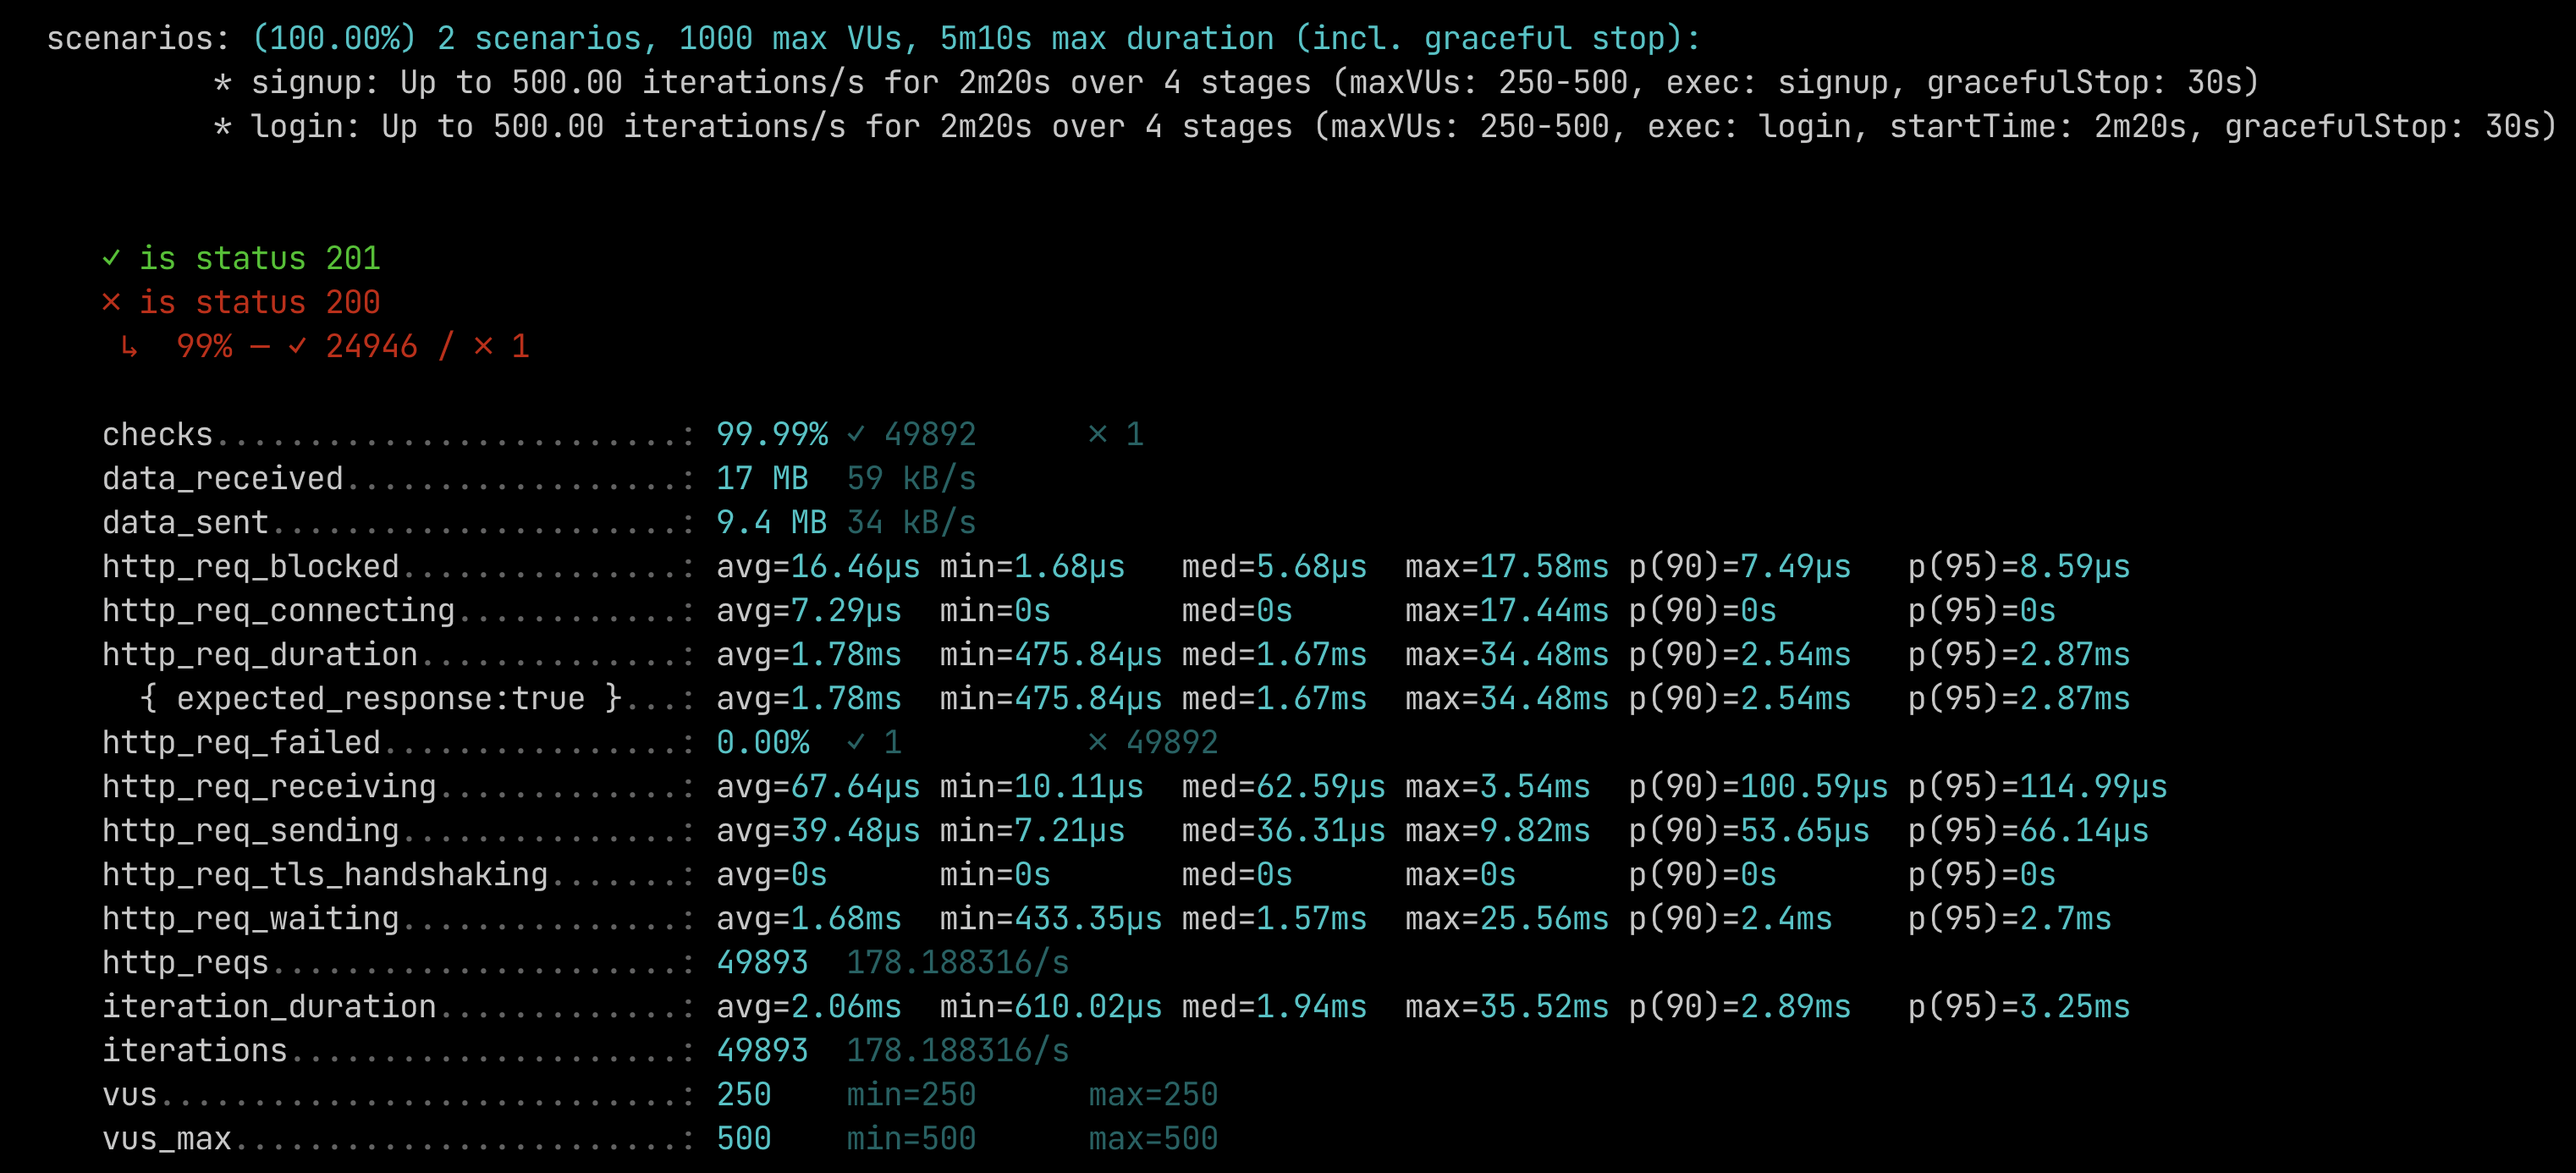
\includegraphics[width=1\linewidth]{figures/k6-ghofl}
	\caption{تست‌بار اجرا شده بر روی میکروسرویس قفل}
	\label{fig:k6-ghofl}
\end{figure}

\begin{figure}
	\centering
	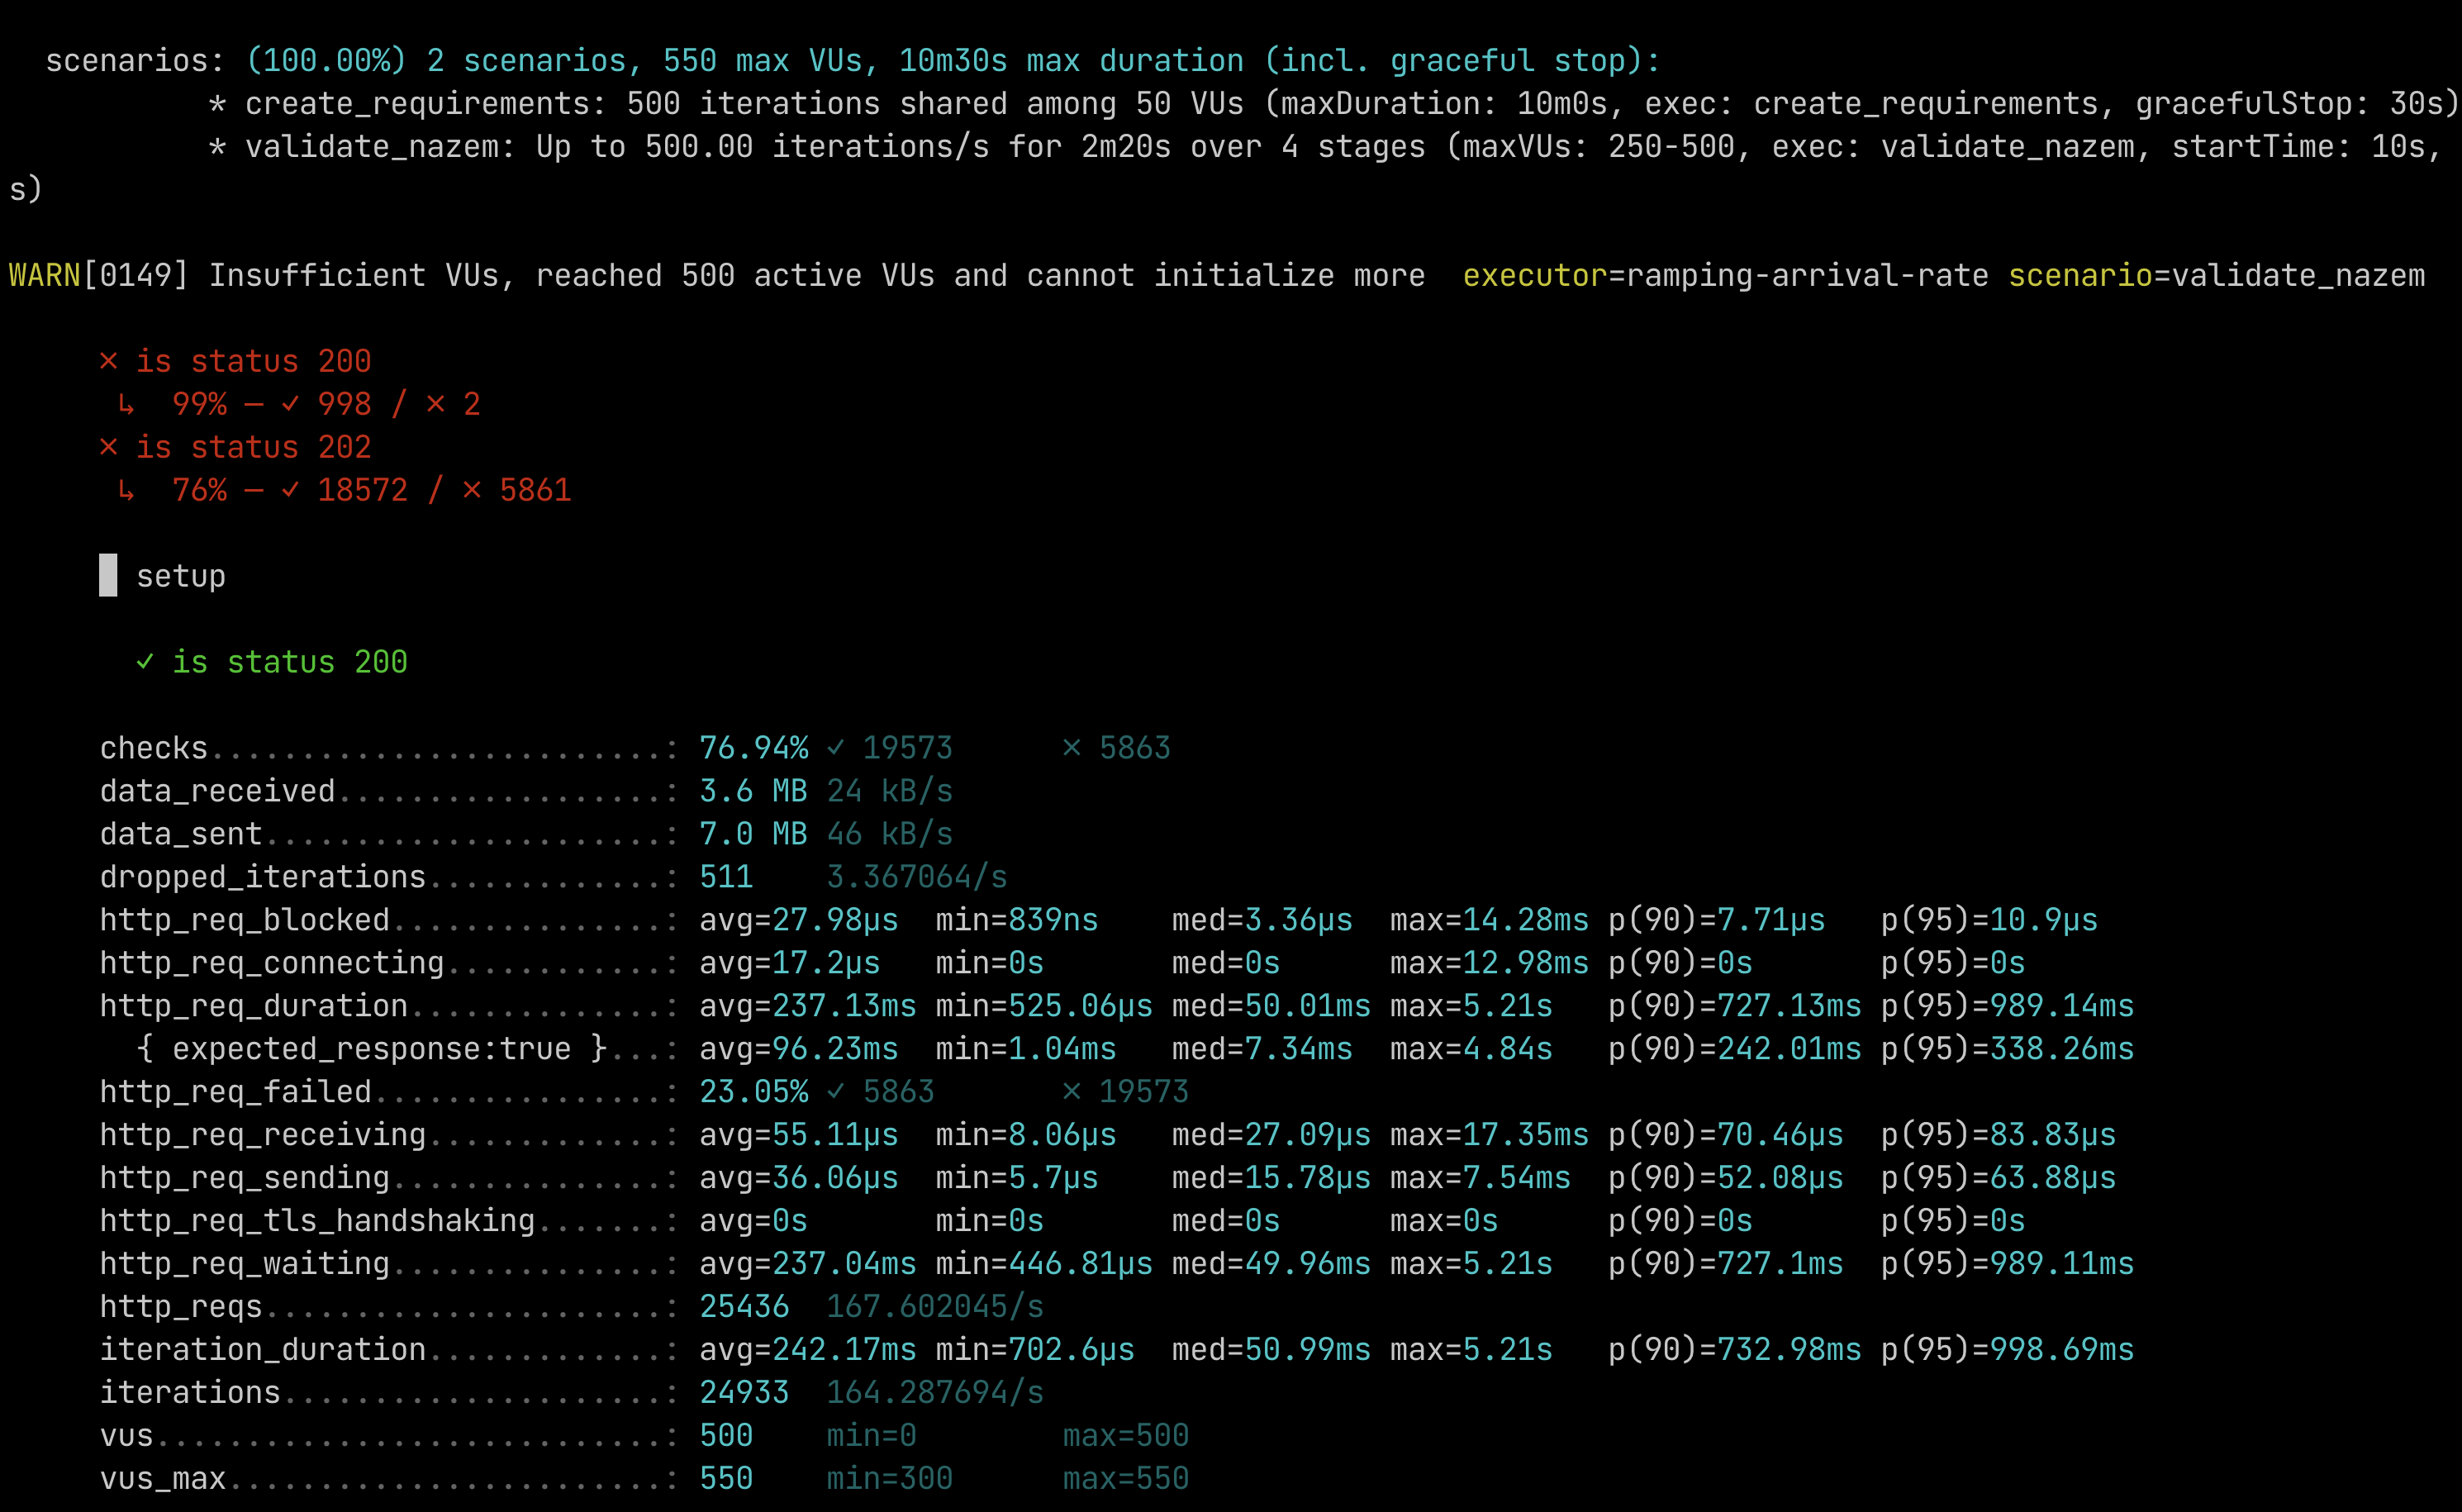
\includegraphics[width=1\linewidth]{figures/k6-nazem}
	\caption{تست‌بار اجرا شده بر روی میکروسرویس ناظم}
	\label{fig:k6-nazem}
\end{figure}



\section{محدودیت‌ها}
با توجه به معماری استفاده‌شده در پیاده‌سازی این سامانه، تمامی خدمت‌گزار‌های سامانه و پایگاه داده می‌توانند به صورت افقی مقیاس شوند تا پاسخگوی حجم‌های احتمالی زیاد باشند. با این وجود بخش‌هایی از سامانه محدودیت‌هایی در راستای حجم فشار کلی سامانه ایجاد می‌کنند.


اولین محدودیت سامانه، عدم امکان مقیاس کردن زمان‌بند سرویس خادم است. این زمان‌بند به صورت مستقیم با کاربران در تعامل نیست و در نتیجه حجم درخواست‌های ناگهانی بار اصلا تاثیرگذار نیست. اما بالا رفتن تعداد منابع ساخته‌شده، یا فشار زیاد شبکه، باعث اختلال در عملکرد و فشار بر این برنامه می‌شود. راه حل کمتر کردن این فشار، رزرو کردن منابع اختصاصی شبکه برای این برنامه در کنار زیاد کردن منابع محاسباتی پیش از اجرا است.

یکی دیگر از محدودیت‌های سامانه که مقیاس شدن برنامه در آن تاثیر کمی دارد، زیرساخت \lr{cloud director} است. با توجه به ساختار تک نسخه‌ای بودن آن در برنامه، تمامی نسخه‌های سرویس خادم با یک نسخه‌از \lr{cloud director} در ارتباط هستند. از آنجایی که عملیات تعریف شده در این برنامه، ذاتا زمان‌بر هستند و نیازمند اجرا به صورت آسنکرون هستند. اجرای حجم زیادی از درخواست‌ها و ارسال آن‌ها به سمت \lr{cloud director} می‌تواند باعث بروز اختلال و اعمال فشار بر این سرویس شود. راه حل پیشنهادی جهت بهبود این محدودیت، تعریف سقف برای تعداد عملیات در حال اجرا در سمت خادم است. این‌کار می‌تواند با قرار دادن یک صف پیام\LTRfootnote{Message Queue} بین سرویس باجه و خادم انجام شود.

\clearpage
